\chapter{De Celsius a Fahrenheit}\label{a:CelsiusFahrenheit}
En aquest capítol mostrarem amb detall la primera xarxa neuronal que vam crear.

Per començar, importem el framework i la biblioteca de Python que són necessàries per a la creació de la xarxa neuronal: \texttt{TensorFlow} (framework) i \texttt{numpy} (biblioteca). Hem creat unes \textit{abreviatures} per poder cridar-les més fàcilment quan es necessitin.

\begin{itemize}
\item \textbf{TensorFlow:} TensorFlow és un framework que ofereix eines per crear i entrenar models de Machine Learning (ML) i Deep Learning (DL), biblioteques per programar xarxes neuronals i altres algoritmes, compatibilitat amb GPU i TPU per accelerar càlculs, TensorBoard per visualitzar i monitorar entrenaments, models preentrenats i repositoris, i APIs en diversos llenguatges.
\item \textbf{numpy:} numpy és una biblioteca científica per treballar amb vectors i matrius.
\end{itemize}

\begin{figure}[H]
\centering
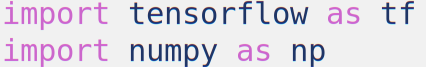
\includegraphics[width=0.3\textwidth]{./figures/1.png}
\caption{Framework i biblioteca de Python}
\end{figure}

Definim les variables \textbf{celsius} i \textbf{fahrenheit} de tipus \texttt{np.array()}, ja que són llistes de valors, i el paràmetre \texttt{dtype=float} per especificar que els valors de la llista són nombres decimals.

Per \textbf{fahrenheit}, les dades no poden ser arbitràries: han de ser les temperatures corresponents a les de \textbf{celsius} convertides a Fahrenheit, de manera que la xarxa neuronal pugui entendre la relació entre ambdues sèries de dades.

\begin{figure}[H]
\centering
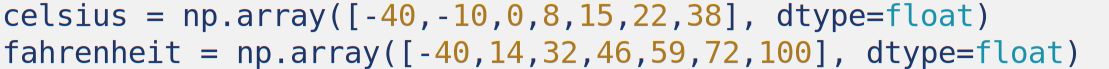
\includegraphics[width=0.7\textwidth]{./figures/2.png}
\caption{Agrupació de dades amb numpy}
\end{figure}

A continuació definim les capes de la xarxa neuronal. Utilitzant \texttt{tf.keras.layers.Dense} (funció per a capes denses), es crea la primera capa oculta amb \texttt{units=3} (3 neurones) i \texttt{input\_shape=[1]} per indicar que l’entrada és un sol valor. La capa rep el nom \texttt{oculte\_1}.

La segona capa oculta, \texttt{oculte\_2}, també té 3 neurones, però no cal especificar \texttt{input\_shape}, ja que la xarxa ho dedueix automàticament de la capa anterior.

Finalment, la capa de sortida té \texttt{units=1} perquè retorni un sol valor (la predicció en Fahrenheit). Amb totes les capes creades, les integrem en un model seqüencial amb \texttt{tf.keras.Sequential}, passant-les dins d’una llista en l’ordre correcte: \texttt{[oculte\_1, oculte\_2, sortida]}. Això crea l’estructura bàsica de la xarxa neuronal.

\begin{figure}[H]
\centering
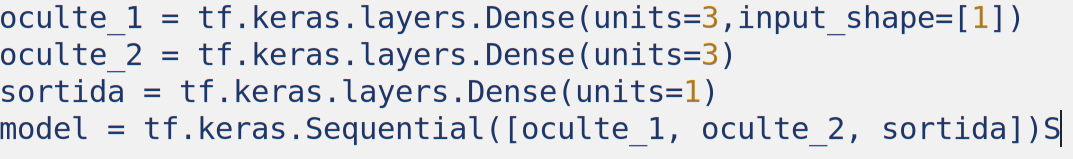
\includegraphics[width=0.7\textwidth]{./figures/3.png}
\caption{Capes ocultes i capa de sortida d’una xarxa neuronal}
\end{figure}

Un cop definida l’estructura, cal ensenyar al model a aprendre i entrenar-se. Utilitzem la variable \textbf{model}, a la qual ja hem assignat les capes. A continuació apliquem \textbf{.compile()} per configurar el model abans de començar l’entrenament.

Dins de \texttt{.compile()} especifiquem \textbf{optimizer}, que indica com el model ajustarà els pesos. En aquest cas utilitzem \texttt{"adam"}, un optimitzador adaptatiu que redueix la velocitat d’aprenentatge quan detecta canvis bruscos en un pes, l’augmenta quan el pes és estable i recorda la direcció correcta per evitar oscil·lacions innecessàries.

Definim la funció de pèrdua (que mesura l'error) amb \textbf{loss="mean\_squared\_error"}. La funció de pèrdua (\textit{loss}) mesura l’error del model i guia l’aprenentatge.
L’opció MSE (Mean Squared Error) penalitza més fortament els errors grans i permet aconseguir prediccions més precises.
$$ MSE = \frac{1}{n} \sum_{i=1}^n \left( x_i - \widehat{x}_i\right)^2$$
% \begin{figure}[H]
% \centering
% 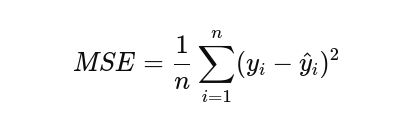
\includegraphics[width=0.5\textwidth]{./figures/5.png}
% \caption{Funció de pèrdua}
% \end{figure}

\begin{figure}[H]
\centering
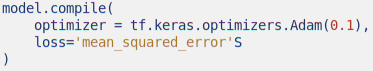
\includegraphics[width=0.5\textwidth]{./figures/4.png}
\caption{Optimització de la xarxa neuronal}
\end{figure}

Per entrenar la xarxa neuronal, utilitzem la variable \texttt{historial} per guardar l’evolució de l’entrenament, aplicant \texttt{.fit()} sobre el model. Dins \texttt{.fit()} indiquem les dades d’entrada (\texttt{celsius}), les dades de sortida (\texttt{fahrenheit}), el nombre de cicles d’entrenament (\texttt{epochs=100}) i si volem mostrar el procés per pantalla (\texttt{verbose=1}).

Podem utilitzar \texttt{print()} per escriure missatges al terminal, com \texttt{"\hspace{0truecm}Comencem a entrenar..."} abans de començar i \texttt{"Model entrenat!"} un cop finalitzat.

\begin{figure}[H]
\centering
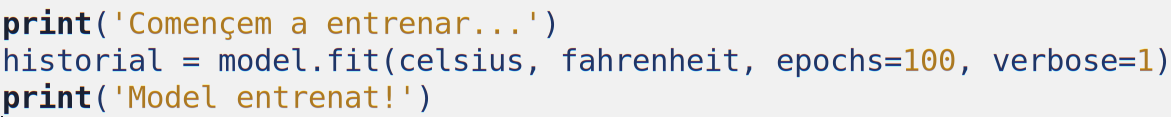
\includegraphics[width=0.7\textwidth]{./figures/6.png}
\caption{L’entrenament de la xarxa neuronal}
\end{figure}

Després d’entrenar la xarxa, podem visualitzar la pèrdua per època amb \texttt{matplotlib.pyplot}. Primer importem la biblioteca amb \texttt{import matplotlib.pyplot as plt} i etiquetem els eixos amb \texttt{plt.xlabel("\# Època")} i \texttt{plt.ylabel("Magnitud de pèrdua")}. La corba es dibuixa amb \texttt{plt.plot(historial.history["loss"])} i es mostra amb \texttt{plt.show()}. Això permet observar si el model aprèn correctament i com disminueix la pèrdua al llarg de les èpoques.

\begin{figure}[H]
\centering
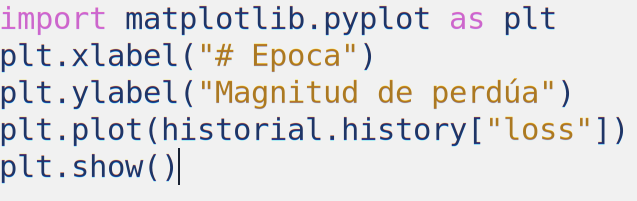
\includegraphics[width=0.4\textwidth]{./figures/7.png}
\caption{Corba de pèrdua}
\end{figure}

Per fer prediccions amb nous valors, utilitzem \texttt{model.predict()}. Per exemple, amb 100 graus Celsius: \texttt{np.array([[100.0]], dtype=float)}. El resultat s’emmagatzema a la variable \texttt{resultat} i es mostra amb \texttt{print("El resultado es " + str(resultat) + " fahrenheit")}.

\begin{figure}[H]
\centering
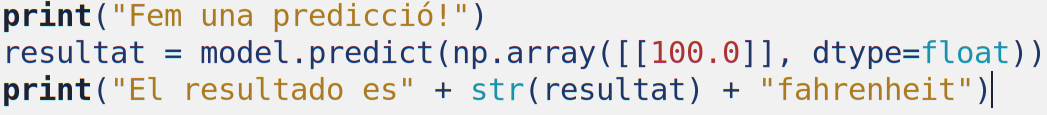
\includegraphics[width=0.7\textwidth]{./figures/8.png}
\caption{Resultat de la predicció}
\end{figure}

Per inspeccionar els pesos interns de la xarxa, utilitzem \texttt{.get\_weights()} en cada capa (\texttt{oculte\_1.get\_weights()}, \texttt{oculte\_2.get\_weights()}, \texttt{sortida.get\_weights()}) i els mostrem amb \texttt{print()}.

\begin{figure}[H]
\centering
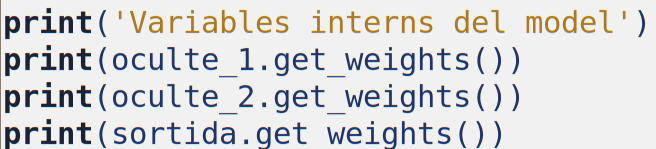
\includegraphics[width=0.4\textwidth]{./figures/9.png}
\caption{Pesos i biaixos assignats}
\end{figure}

Finalment, es mostren exemples de l’inici de l’entrenament, del model entrenat, de la gràfica de pèrdua i del resultat de la predicció amb 100 Celsius:

\begin{minipage}{0.45\textwidth}
  \begin{figure}[H]
  \centering
  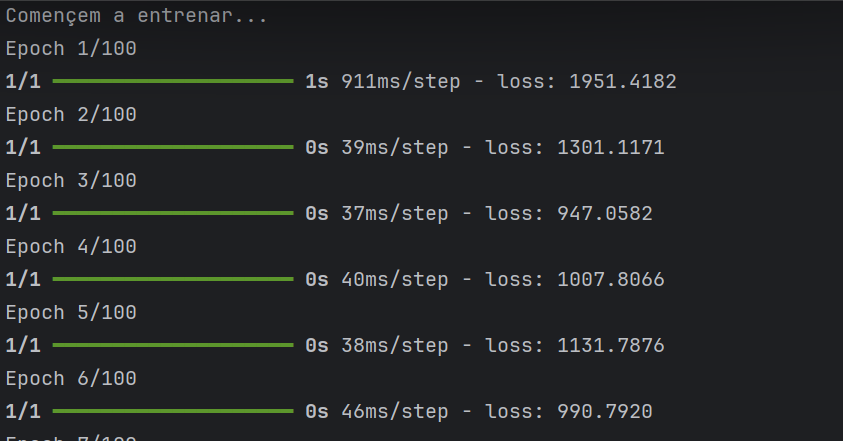
\includegraphics[width=1\textwidth]{./figures/10.png}
  \caption{Inici de l’entrenament}
  \end{figure}
\end{minipage}
\begin{minipage}{0.45\textwidth}
\begin{figure}[H]
\centering
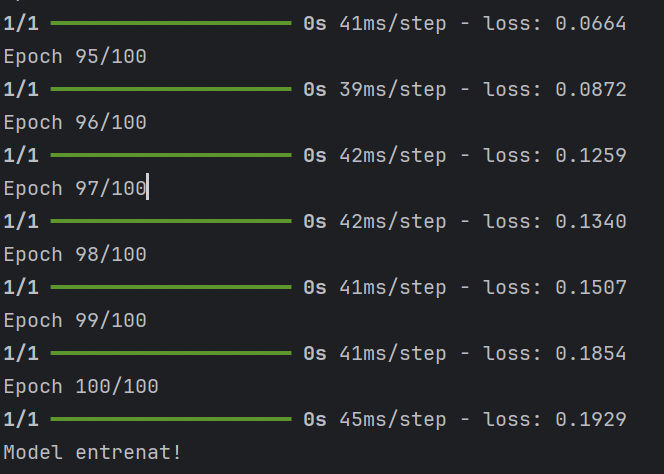
\includegraphics[width=0.9\textwidth]{./figures/11.png}
\caption{Model entrenat}
\end{figure}
\end{minipage}

\begin{figure}[H]
\centering
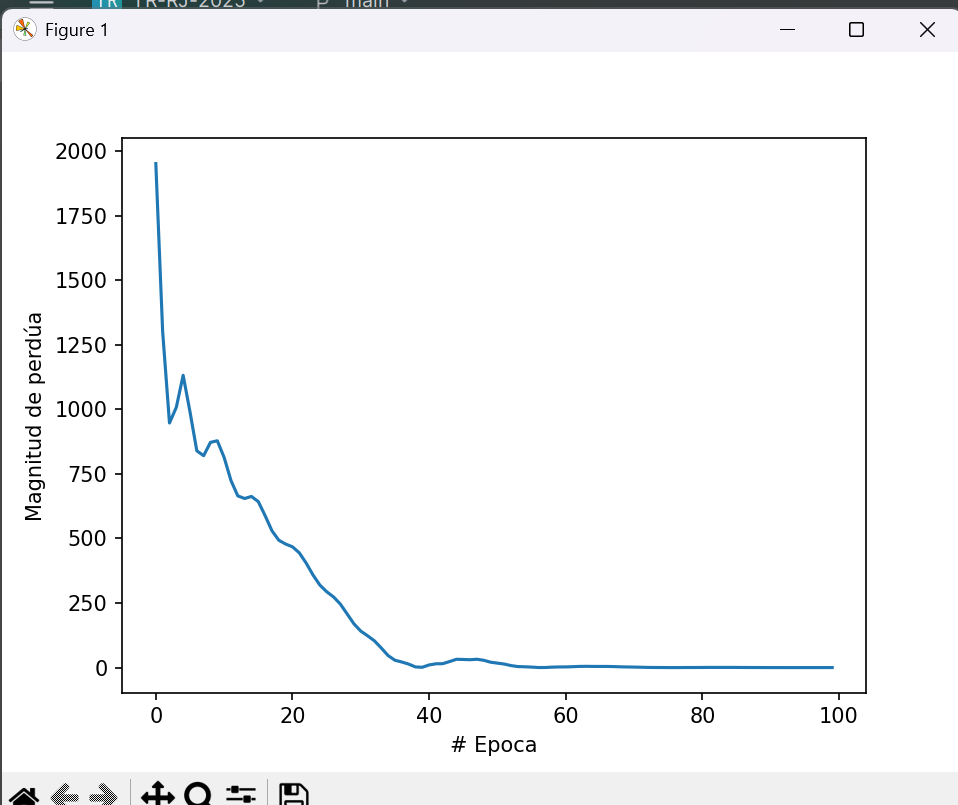
\includegraphics[width=0.5\textwidth]{./figures/12.png}
\caption{Gràfica de la corba de pèrdua}
\end{figure}

\begin{figure}[H]
\centering
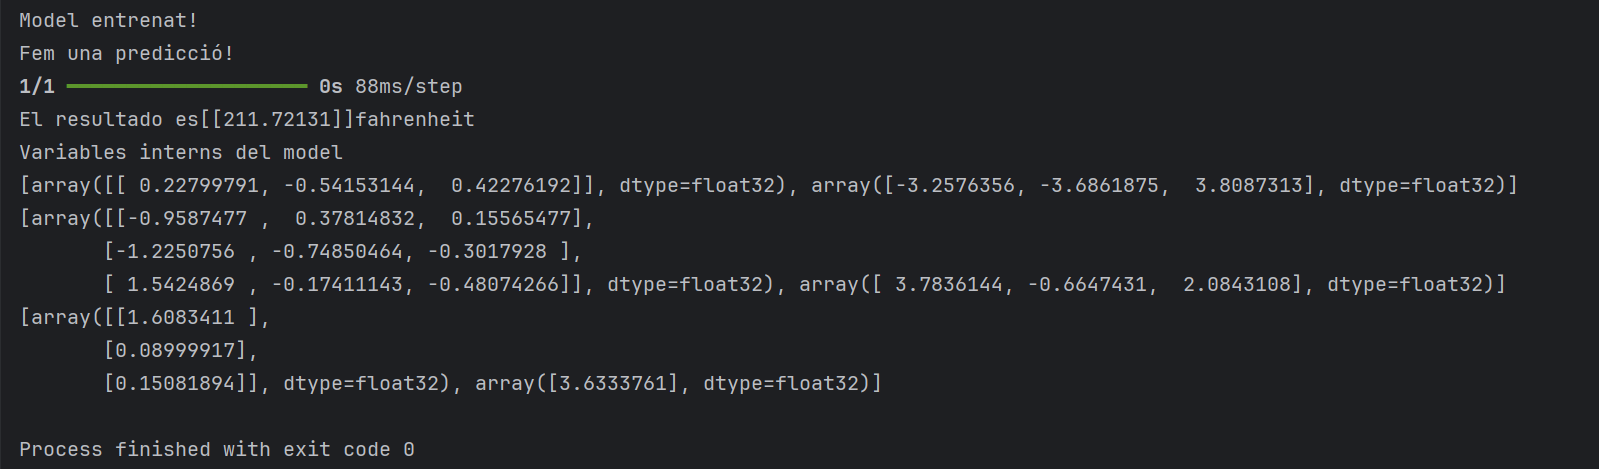
\includegraphics[width=0.9\textwidth]{./figures/13.png}
\caption{Resultat de la predicció i pesos utilitzats per la xarxa neuronal}
\end{figure}

Podeu trobar el codi complet al respositori del nostre TR~\cite{TR-RJ-2025}

Font: \cite{Xarxa_Neuronal}
